\documentclass{article}

\usepackage{tikz}
\usetikzlibrary{braids}

\begin{document}
\begin{figure}[h]
\caption{For every content strand, the four proficiency strands are inter-twined.}
\label{fig:proficiency strands}
\begin{center}
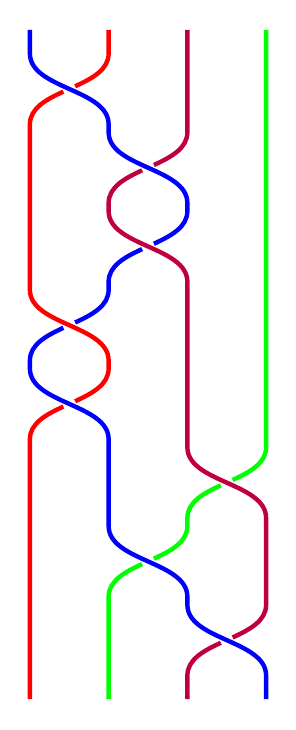
\begin{tikzpicture}
%
\pic[
  ultra thick,
  braid/strand 1/.style={blue},
  braid/strand 2/.style={red},
  braid/strand 3/.style={purple},
  braid/strand 4/.style={green}
]
(profs)
{braid={
s_1 s_2
s_2 s_1
s_1 s_3
s_2 s_3
}};
\end{tikzpicture}
\end{center}
\end{figure}
\end{document}


\documentclass{article}

\usepackage{tikz}
\usepackage{braids}

\begin{document}

\begin{figure}[h]
\caption{For every content strand, the four proficiency strands are inter-twined.}
\label{fig:proficiency strands}
\begin{center}
\begin{tikzpicture}
%
\braid[
number of strands=3,
style strands={1}{blue, ultra thick},
style strands={2}{red, ultra thick},
style strands={3}{purple, ultra thick},
style strands={4}{green, ultra thick}
]
(profs)
s_1 s_2
s_2 s_1
s_1 s_3
s_2 s_3;
\end{tikzpicture}
\end{center}
\end{figure}

\end{document}
